\documentclass[11pt]{article}
\usepackage[margin=1in]{geometry}
\usepackage[T1]{fontenc}
\usepackage{lmodern}
\usepackage{microtype}
\usepackage{booktabs}
\usepackage{amsmath,amssymb}
\usepackage{graphicx}
\usepackage{hyperref}
\usepackage[numbers,sort&compress]{natbib}
\usepackage{caption}
\captionsetup{font=small}

\title{Few-Label Transfer Across Network Flow Datasets: Meta-Training on Network Tasks Versus a Tabular Foundation Model}
\author{Quang-Vinh Dang\\
British University Vietnam, Hung Yen, Vietnam\\
\texttt{vinh.dq4@buv.edu.vn}\quad ORCID 0000-0002-3877-8024}
\date{}

\begin{document}
\maketitle

\begin{abstract}
Flow-based intrusion detectors that score above 0.99 ROC-AUC inside one dataset often fall to chance on another.
On eight public flow datasets from five laboratories, no flow feature keeps the same direction of association with the attack label, and a classifier trained on the pooled other datasets reaches only 0.32 to 0.95 ROC-AUC on a held-out one; in a companion benchmark, domain-adaptation methods and our own transfer method did not significantly improve on a plain gradient-boosted baseline.
We therefore ask what can be learned from other networks when only $k=4$ to $128$ target flows are labelled.
We build FLARE-2, a transformer meta-trained on episodes from the other datasets that reads the detection rule from the labelled flows at test time, and compare it with tree ensembles and with TabPFN versions 3 and 3.5, general-purpose tabular foundation models that we did not train or tune on network data.
Over eight targets and three meta-training seeds, FLARE-2 shows no significant difference from random forest and CatBoost on binary ROC-AUC ($+0.001$ and $-0.001$, 95\% intervals within $\pm0.006$), but TabPFN-3.5 is higher than FLARE-2 on every target (mean difference $-0.014$, 95\% interval $[-0.018,-0.011]$), higher than random forest on all targets and than target-only CatBoost on 7 of 8 (seed 0, uncorrected $p=0.008$ and $0.016$).
In our experiments, meta-training on real network tasks therefore did not improve on a general-purpose pretrained prior at binary detection.
At attack-class level FLARE-2 has higher per-class ROC-AUC than random forest and CatBoost ($+0.011$, 7 of 8 targets, $p_{\text{Holm}}=0.047$) and a lower false-positive rate, at lower recall at threshold 0.5 and lower $N$-way balanced accuracy than CatBoost; TabPFN-3.5 is not different from FLARE-2 in per-class ROC-AUC ($-0.002$) or $N$-way macro-F1 at class level and has higher recall (seed 0).
We also report where FLARE-2 does not help: source-pretrained CatBoost has higher mean ROC-AUC at $k=4$ on four targets (no significant difference), and FLARE-2 is not better than trees fitted on the target labels at $k\ge32$.
Code, configurations and all raw per-run results are public.
\end{abstract}

\section{Introduction}
Machine-learning intrusion detection on network flows is usually evaluated by splitting one dataset into train and test.
Under that protocol, gradient-boosted trees reach ROC-AUC above 0.99 on CIC-IDS2017, USB-IDS-1 and similar sets.
Studies that move the same model to a second dataset report a collapse \citep{layeghy2023explainable,cantone2024crossdataset,dhooge2020inter,apruzzese2022cross}, and a line of work asks whether domain adaptation helps \citep{layeghy2023dinids}.
An earlier study of ours trained on one dataset, measured the distance of a new dataset to it with an isolation-forest score, and fine-tuned CatBoost on labelled target rows \citep{dang2023learning}.
That approach needs target labels, and we show below that, on average, source pre-training does not beat training on the target labels alone.

This paper builds on the diagnosis and asks what source data can still contribute when a few target flows are labelled.
We make four contributions.
\begin{enumerate}
\item \textbf{Evidence consistent with a change of the labelling function between datasets (concept shift), not only of feature scales.}
On eight datasets from five laboratories and three flow extractors, no common flow feature keeps its sign of association with the attack label (0 of 14), a domain classifier recognises the source dataset of a flow with 91.5\% accuracy among the seven core datasets, and a pooled-source CatBoost reaches 0.32--0.95 ROC-AUC on the held-out dataset.
\item \textbf{FLARE-2}, a few-label meta-learner for flow data trained on tasks from other networks.
It is permutation-invariant over features, accepts any feature set, and handles binary detection and attack-type classification with the same readout.
\item \textbf{A comparison with a tabular foundation model, which is the main empirical finding.}
TabPFN versions 3 and 3.5, general-purpose models that we did not train or tune on network data (the model card of version 3 states that it is trained purely on synthetic tabular tasks \citep{priorlabs2026tabpfn3}), are better than FLARE-2 on binary ROC-AUC on every target (mean over $k$) by 0.008 (TabPFN-3, seed 0) to 0.014 (TabPFN-3.5, three seeds), and TabPFN-3.5 is above random forest on all targets.
\item \textbf{A paired evaluation at the level of the target dataset and the attack class}, with exact Wilcoxon tests, bootstrap intervals over targets, three meta-training seeds, controls for the normalisation and for in-context behaviour, and a candid account of the cases FLARE-2 loses.
\end{enumerate}
We do not claim that FLARE-2 is the best few-label method: it matches fixed-setting tree ensembles on binary ROC-AUC and a general-purpose foundation model is better.
What the study supports is that a few labelled flows of the target network, combined with a strong pretrained prior, are the reliable ingredient, and that, in our experiments, meta-training on real network tasks did not improve on that prior at the binary level.

\section{Related work}
\paragraph{Cross-dataset intrusion detection.}
\citet{layeghy2023explainable} train on one NetFlow-v2 dataset and test on another and report attack-class F1 below 1\% for several pairs; \citet{cantone2024crossdataset} report MCC around 0.3 between CIC-IDS2017 and CIC-IDS2018; \citet{dhooge2020inter,dhooge2023damaged} study generalisation per attack class; \citet{apruzzese2022cross} cross-evaluate detectors across datasets and \citet{engelen2021troubleshooting} document labelling errors in CIC-IDS2017; \citet{arp2022dos} and \citet{apruzzese2023sok} discuss pitfalls of ML evaluation in security.
\citet{sarhan2022standard} propose standard NetFlow feature sets to ease cross-dataset use.
Domain-invariant training \citep{layeghy2023dinids}, built on adversarial alignment \citep{ganin2016dann} or covariance alignment \citep{sun2016coral}, assumes the labelling function is shared.
Our controls probe that assumption but cannot isolate concept shift from a change of attack mix.
\paragraph{Few-shot and in-context learning.}
Matching and prototypical networks \citep{vinyals2016matching,snell2017prototypical} and gradient-based meta-learning \citep{finn2017maml} learn from episodes.
Prior-fitted networks \citep{muller2022pfn} and TabPFN \citep{hollmann2025tabpfn} fit a transformer to synthetic tabular tasks and classify by attention to the labelled rows.
FLARE-2 follows this in-context recipe but meta-trains on \emph{real} tasks from other networks, adds a task distribution designed for the cross-network case, and uses a matching readout that fits a variable label space.
We also evaluate TabPFN itself, versions 3 and 3.5, on the same supports, which tests whether meta-training on network tasks adds anything to a model pretrained on synthetic tasks only.
Set-based architectures \citep{lee2019settransformer} motivate our permutation invariance over rows and features.

\section{Problem, data and evidence of concept shift}
\subsection{Datasets and common flow schema}
Table~\ref{tab:data} lists the eight datasets.
Several datasets share a laboratory (CIC-IDS2017 and CIC-IDS2018, UNSW-NB15 and ToN-IoT, IoT-23 and CTU-13), so the eight datasets come from five laboratories and use three extractors (CICFlowMeter, Argus, Zeek).
Extractors export different features, so we keep only features of the same physical meaning and units: five base features (duration, forward and backward packets, forward and backward bytes) plus eight derived rates and ratios (13 in the core tier used by FLARE-2; the sign analysis below adds \texttt{bytes\_per\_pkt} from the minimal tier and so uses 14), all passed through $\log(1+x)$.
CTU-13 supports only a nine-feature minimal tier (four base features and five derived); FLARE-2 takes it as a target without change because it accepts any number of features.
Ports and protocol are excluded.
Rows are sampled by a seeded 64-bit hash of the harmonised features and label (a bottom-$k$ sketch), which gives a uniform sample of distinct rows; the attack prior is that of the distinct rows.

\begin{table}[t]
\centering\small
\caption{Datasets. Extractor: CIC = CICFlowMeter.}\label{tab:data}
\begin{tabular}{llll}
\toprule
Dataset & Laboratory & Extractor & Reference\\
\midrule
CIC-IDS2017 & UNB CIC & CIC & \citep{sharafaldin2018cicids}\\
CIC-IDS2018 & UNB CIC / CSE & CIC & \citep{sharafaldin2018cicids}\\
USB-IDS-1 & Univ.\ of Sannio & CIC & \citep{catillo2021usbids1}\\
InSDN & Univ.\ College Dublin & CIC & \citep{elsayed2020insdn}\\
UNSW-NB15 & UNSW Canberra & Argus & \citep{moustafa2015unsw}\\
ToN-IoT & UNSW Canberra & Zeek & \citep{alsaedi2020toniot}\\
IoT-23 & Stratosphere Lab, CTU & Zeek & \citep{garcia2020iot23}\\
CTU-13 & Stratosphere Lab, CTU & Argus & \citep{garcia2014ctu13}\\
\bottomrule
\end{tabular}
\end{table}

\subsection{Setting}
We use leave-one-dataset-out (LODO): the target dataset is never seen in meta-training or checkpoint selection.
At test time a method receives a support set of $k\in\{4,8,16,32,64,128\}$ labelled target flows with at least one flow per class, and may use no other target label. FLARE-2 additionally ranks features over the unlabelled target rows it scores (Sect.~\ref{sec:method}); the baselines receive no such information.
Support sets are drawn 10 times per $(\text{target},k)$ with fixed seeds and are identical for every method.
Evaluation is on the target test split.
For class level we use $k\in\{2,4,8,16\}$ labelled flows \emph{per class} and 5 draws (InSDN only up to $k=8$ per class, because its attack classes are small).

\subsection{Why transfer fails: three controls}\label{sec:shift}
\paragraph{No stable feature direction.}
For each of the 14 common features we compute the ROC-AUC against the attack label inside every dataset.
None has AUC above 0.5 in all datasets or below 0.5 in all datasets (0 of 14 consistent; e.g.\ \texttt{total\_bytes} ranges from 0.025 to 0.760).
\paragraph{Datasets are identifiable.}
A CatBoost domain classifier recognises the source dataset of a flow with 91.5\% accuracy on seven datasets (chance 14.3\%), 91.8\% on benign flows alone.
A model given unlabelled context can therefore recognise which dataset it is in and apply a memorised rule; our first attempt with unlabelled context rows failed for this reason (Sect.~\ref{sec:method}).
\paragraph{Source pre-training does not help the target.}
Over 42 source--target pairs, a source-pretrained CatBoost fine-tuned on 0.1\% of target labels reaches 0.835 ROC-AUC, below the 0.928 of CatBoost trained on those labels alone; with 300 or 500 extra trees the gap narrows (0.911 vs 0.932) but does not close.
Table~\ref{tab:zero} shows the zero-shot picture: a CatBoost trained on all other datasets (LODO) scores from 0.322 (IoT-23) to 0.952 (USB-IDS-1), below chance on three targets (IoT-23, CTU-13, UNSW-NB15).

\begin{table}[t]
\centering\small
\caption{Zero-shot ROC-AUC on the target test split ($k=0$). LODO: CatBoost on all other datasets pooled. Pairwise: mean and best single source from the pairwise benchmark (not computed for CTU-13). Full label: CatBoost trained on the full target train split.}\label{tab:zero}
\begin{tabular}{lcccc}
\toprule
Target & CatBoost LODO & pairwise mean & pairwise best & full label \\
\midrule
CIC-IDS2017 & 0.832 & 0.559 & 0.761 & 0.999 \\
CIC-IDS2018 & 0.656 & 0.547 & 0.698 & 0.968 \\
CTU-13 & 0.358 & -- & -- & 0.962 \\
InSDN & 0.730 & 0.598 & 0.827 & 0.998 \\
IoT-23 & 0.322 & 0.370 & 0.460 & 0.950 \\
ToN-IoT & 0.608 & 0.593 & 0.942 & 0.999 \\
UNSW-NB15 & 0.485 & 0.585 & 0.781 & 0.977 \\
USB-IDS-1 & 0.952 & 0.695 & 0.965 & 1.000 \\
\bottomrule
\end{tabular}

\end{table}

\section{Method}\label{sec:method}
FLARE-2 classifies a query flow by attending to labelled support flows of the same episode.
At test time the episode is the $k$ support flows and the query flows; nothing is trained.

\paragraph{Episode normalisation.}
Within an episode, each feature is mapped to its Gaussian rank over support and query rows and clipped to $[-4,4]$. At test time the query rows are the whole unlabelled target test split (and, for per-class evaluation, only the rows of the class and of benign), whereas training episodes rank over 256 query rows, so FLARE-2 is transductive in the target features and the per-class pool depends on the class labels of the test rows. A control with a reference of 256 query rows, as in training, gives the same ROC-AUC (Sect.~\ref{sec:controls}).
Absolute scales, which differ across extractors, therefore never reach the network.
Missing features are absent tokens.

\paragraph{Tokens and layers.}
Flow $i$ with features $x_{i1},\dots,x_{id}$ becomes $d$ feature tokens $t_{ij}=\mathrm{MLP}_v(x_{ij})$ with a shared scalar embedding, plus one label token.
There is no feature-identity embedding, so the model cannot memorise that ``feature 7 high means attack'' and is invariant to feature order.
Six layers of width 128 with 4 heads alternate \emph{feature attention} (tokens of one row attend to each other) and \emph{row attention} (rows attend across the episode).
Support rows attend to support rows; a query row attends to support rows and itself only, so attention does not depend on which other queries share the batch; the rank normalisation above does.

\paragraph{Label slots and matching readout.}
Class identities differ between episodes, so each support class is given a random one of $M=16$ label-slot embeddings as input.
The readout does not index slots.
Each row is summarised by the layer-normalised mean $r_i$ of its tokens; a query gives $q=W_q r$, a support row $s$ gives key $k_s=W_k r_s$, and the logit of an active class $j$ with support $S_j$ is
\begin{equation}
\ell_j=\log\!\!\sum_{s\in S_j}\exp\!\Big(\frac{\langle q,k_s\rangle}{\sqrt{w}\,\tau}\Big)-b\log|S_j|,
\end{equation}
with $w=128$, a learned temperature $\tau>0$ and a learned $b\in[0,1]$ that interpolates between sum and mean pooling over a class's keys.
A softmax over the $N$ active classes is trained with cross-entropy.
The head is equivariant to permutations of classes and slots by construction and serves binary detection ($N=2$) and attack-type classification alike.
A slot-indexed linear head plateaued in training and was replaced by this one.
At test time we average class logits over 8 members with different sign flips and class-to-slot maps.

\paragraph{Meta-training episodes.}
Each episode draws a source dataset (weighted by $\sqrt{\text{size}}$) and a \emph{task}: binary attack vs benign (probability 0.25), one attack class vs benign (0.25), class vs class (0.15), or $N$-way with $N\sim U\{3..6\}$ among benign and attack classes (0.35).
Raw attack types with fewer than 30 rows are dropped.
The per-class support size is log-uniform on $\{1,\dots,32\}$ with at most 160 support rows in total, so a binary episode never has more than 64 support rows while evaluation uses up to 128; the query class proportions are Dirichlet(1) with at least one query row per class, so no fixed prior can be learned; 30\% of binary, one-class and $N$-way episodes (about 25\% of all episodes) combine benign rows of one dataset with attack classes of another; with probability 0.5 a random subset of at least 5 features is kept; 2\% of support labels are flipped; each feature is sign-flipped independently with probability 0.5.
A monotone warp was also tried; it has no effect under rank normalisation and was dropped.
Because both the meaning of a class and the sign of every feature change from episode to episode, the only reliable strategy is to read the rule from the support set.
This is the design response to the concept shift of Sect.~\ref{sec:shift}; Sect.~\ref{sec:ablation} measures how much the individual choices, including the class-level tasks, contribute, and the evidence for them is modest.

\paragraph{Held-out-source model selection.}
Our first variant added unlabelled context rows from the target network.
It reached 0.97 AUC on validation episodes from the meta-training datasets but fell to 0.66--0.76 on the unseen IoT-23 target: with datasets identifiable at 91\%, six binary tasks are easy to memorise.
In FLARE-2, one source dataset (rotating, never the target) is excluded from training and used only to select the checkpoint with the lowest validation loss.
The unlabelled-context variant is not part of FLARE-2.

\paragraph{Training.}
AdamW (learning rate $3\times10^{-4}$, weight decay 0.01, cosine schedule, 1k warm-up steps), 20k steps, 8 episodes per step, 256 query rows, gradient clipping at 1.0, mixed-precision autocast (fp16 on a Colab T4 for the main runs, bf16 on a local RTX GPU for the ablation runs and extra seeds).
One model is trained per target (LODO), about 1 hour each.
The label-slot readout computes in float32 to avoid half-precision overflow.

\section{Experimental protocol}
\paragraph{Baselines on identical supports.}
Random forest (RF), CatBoost \citep{prokhorenkova2018catboost}, logistic regression (LR) and $k$NN trained on the $k$ target labels only; CatBoost pretrained on the sources and fine-tuned on the $k$ labels (the earlier approach); and, as zero-shot references, CatBoost trained on all other datasets and the pairwise single-source results.
Baselines use fixed standard settings and no tuning (RF: 300 trees; CatBoost: 300 iterations, depth 6, learning rate 0.05; LR and $k$NN with up to 5 neighbours on standardised features; class-balanced weights), since selecting hyperparameters from a handful of labels is itself unreliable; a baseline tuned with extra target labels could be stronger.
For $N$-way, baselines are the multi-class versions trained on the labelled $k$ per class.
\paragraph{Tabular foundation models.}
TabPFN \citep[the family of][]{hollmann2025tabpfn}, versions 3 and 3.5 (released weights of the \texttt{tabpfn} package, version 9.2.0, and of the \texttt{Prior-Labs/tabpfn\_3} repository), with default settings and the same support and query rows as every other method.
We did not train or tune the models on network data (the model card of version 3 states that it is trained purely on synthetic tabular tasks \citep{priorlabs2026tabpfn3}; we have not verified the pretraining data of version 3.5); they read the support set as training data and score each query row independently of the other query rows, so, unlike FLARE-2, they do not use the unlabelled target rows.
Version 3.5 was run for all three meta-training seeds and version 3 for seed 0.
At class level TabPFN-3.5 was run for seed 0 with five draws (the draws of FLARE-2): on all query rows of IoT-23, ToN-IoT and CTU-13, and, to save time, on a fixed stratified subsample of at most 5\,000 query rows per task for the other five targets; scoring IoT-23 both ways changes the class-level metrics by at most 0.005 on average (per-class ROC-AUC $+0.002$, macro-F1 $+0.001$, recall $+0.005$).
The weights are released under a non-commercial research license, which applies here.
\paragraph{Metrics and statistics.}
ROC-AUC (binary and per class), recall and false-positive rate at threshold 0.5, and macro-F1 for $N$-way classification.
Draws of one target are not independent, so the unit of analysis is the \emph{target}: the mean difference of FLARE-2 minus baseline over draws, then an exact two-sided Wilcoxon signed-rank test over the 8 targets (smallest attainable $p=0.0078$), Holm-adjusted over the five baselines (four at class level in the three-seed analysis; Table~\ref{tab:class} reports uncorrected seed-0 $p$), and a 95\% bootstrap interval over targets. Only the mean over $k$ is a primary endpoint; the $k\le16$ and $k\ge32$ splits are exploratory.
For class-level results we also report units of (target, class), with a warning that classes of one target are correlated; the target-level test is the conservative one.

\section{Results}
\subsection{Binary detection}
Table~\ref{tab:binary} and Fig.~\ref{fig:curves} show ROC-AUC versus $k$.
With $k=4$ labelled flows, FLARE-2 already beats the zero-shot pooled CatBoost on five of eight targets (CTU-13, IoT-23, ToN-IoT, UNSW-NB15, USB-IDS-1; Tables~\ref{tab:zero},~\ref{tab:binary}); on the other three (CIC-IDS2017, CIC-IDS2018, InSDN), where pooled sources transfer well, 8 to 16 labelled flows are needed to catch up.
Table~\ref{tab:stats} gives the paired statistics.
Against the strongest baselines the difference is small and not significant: mean over $k$, FLARE-2 minus target-only CatBoost is $-0.001$ and minus RF is $+0.004$; both intervals contain zero and the win/loss counts over targets are 4/4 and 5/3.
Against LR and $k$NN the gain is large: FLARE-2 is higher on all 8 targets for the mean over $k$ ($+0.075$ and $+0.110$, $p_{\text{Holm}}=0.039$ for both).
Against source-pretrained CatBoost fine-tuned on the labels, seed 0 shows FLARE-2 better for $k\ge 32$ (7 of 8 targets, $p_{\text{Holm}}=0.047$) and not different below; the repeat over seeds below shows that this advantage is not robust.

\paragraph{Three meta-training seeds.}
We repeated the benchmark (meta-training, the split of the target and the support draws) with seeds 1 and 2 on all eight targets, for FLARE-2 and every baseline.
Table~\ref{tab:seeds} gives the paired differences with the target as unit, after averaging each target over the three seeds.
The seed-averaged differences to RF and to target-only CatBoost are $+0.001$ and $-0.001$ for the mean over $k$ (per seed $-0.002$ to $+0.004$), and the standard deviation over seeds of the mean difference is 0.001 to 0.009 across the rows of Table~\ref{tab:seeds}, so training variance is small next to the spread between targets.
FLARE-2 stays above LR and $k$NN on all 8 targets in every scope ($p_{\text{Holm}}=0.039$).
The seed-0 advantage over fine-tuned CatBoost at $k\ge 32$ shrinks to $+0.007$ (5 of 8 targets, $p_{\text{Holm}}=0.33$), and the mean difference over $k$ is $+0.002$ (CI $[-0.015,+0.020]$).
We therefore claim neither superiority nor inferiority to the tree ensembles on binary ROC-AUC.

\begin{table}[t]
\centering\small
\caption{FLARE-2 minus baseline in binary ROC-AUC, mean over meta-training seeds 0--2, unit = target (8). W/L: targets where FLARE-2 is higher / lower. SD: standard deviation over seeds of the mean difference. $p_{\text{Holm}}$: exact Wilcoxon over targets, Holm-adjusted over the five baselines within each scope. Only the mean over $k$ is a primary endpoint.}\label{tab:seeds}
\resizebox{\linewidth}{!}{\begin{tabular}{llrrrrr}
\toprule
Scope & Baseline & Mean diff. & 95\% CI & W/L & SD over seeds & $p_{\text{Holm}}$ \\
\midrule
mean over k & RF & +0.001 & [-0.004, +0.006] & 4/4 & 0.003 & 1.000 \\
 & CatBoost (target only) & -0.001 & [-0.004, +0.002] & 4/4 & 0.001 & 1.000 \\
 & CatBoost (source + fine-tune) & +0.002 & [-0.015, +0.020] & 3/5 & 0.004 & 1.000 \\
 & LR & +0.073 & [+0.044, +0.102] & 8/0 & 0.003 & 0.039 \\
 & kNN & +0.113 & [+0.090, +0.135] & 8/0 & 0.004 & 0.039 \\
\midrule
k$\leq$16 & RF & +0.002 & [-0.006, +0.012] & 3/5 & 0.003 & 1.000 \\
 & CatBoost (target only) & -0.002 & [-0.008, +0.004] & 3/5 & 0.001 & 1.000 \\
 & CatBoost (source + fine-tune) & -0.004 & [-0.034, +0.030] & 3/5 & 0.003 & 1.000 \\
 & LR & +0.082 & [+0.046, +0.118] & 8/0 & 0.005 & 0.039 \\
 & kNN & +0.174 & [+0.131, +0.215] & 8/0 & 0.009 & 0.039 \\
\midrule
k$\geq$32 & RF & -0.001 & [-0.004, +0.004] & 2/6 & 0.003 & 1.000 \\
 & CatBoost (target only) & -0.000 & [-0.003, +0.002] & 3/5 & 0.003 & 1.000 \\
 & CatBoost (source + fine-tune) & +0.007 & [+0.002, +0.012] & 5/3 & 0.005 & 0.328 \\
 & LR & +0.064 & [+0.035, +0.095] & 8/0 & 0.005 & 0.039 \\
 & kNN & +0.051 & [+0.037, +0.066] & 8/0 & 0.005 & 0.039 \\
\bottomrule
\end{tabular}
}
\end{table}

\begin{table}[t]
\centering\scriptsize
\caption{Binary ROC-AUC, mean over 10 support draws. F2: FLARE-2; RF: random forest; CB: CatBoost on target labels; CB-ft: source-pretrained CatBoost fine-tuned on the labels. TP3.5: TabPFN-3.5. Bold marks the best of the five.}\label{tab:binary}
\resizebox{\textwidth}{!}{\begin{tabular}{lccccccccccccccc}
\toprule
& \multicolumn{5}{c}{$k=4$} & \multicolumn{5}{c}{$k=16$} & \multicolumn{5}{c}{$k=64$} \\
\cmidrule(lr){2-6}\cmidrule(lr){7-11}\cmidrule(lr){12-16}
Target & F2 & RF & CB & CB-ft & TP3.5 & F2 & RF & CB & CB-ft & TP3.5 & F2 & RF & CB & CB-ft & TP3.5 \\
\midrule
CIC-IDS2017 & 0.785 & 0.718 & 0.754 & \textbf{0.841} & 0.747 & 0.861 & \textbf{0.888} & 0.861 & 0.880 & 0.887 & 0.965 & 0.966 & 0.969 & 0.956 & \textbf{0.979} \\
CIC-IDS2018 & 0.605 & 0.599 & 0.604 & \textbf{0.691} & 0.611 & 0.695 & 0.657 & 0.711 & \textbf{0.733} & 0.713 & 0.892 & 0.884 & 0.880 & 0.875 & \textbf{0.904} \\
CTU-13 & 0.599 & 0.599 & 0.599 & 0.470 & \textbf{0.633} & 0.704 & 0.700 & \textbf{0.718} & 0.648 & 0.709 & 0.797 & 0.806 & 0.797 & 0.783 & \textbf{0.807} \\
InSDN & 0.644 & 0.671 & 0.690 & \textbf{0.804} & 0.659 & 0.901 & 0.872 & 0.875 & 0.890 & \textbf{0.911} & 0.960 & 0.956 & 0.954 & 0.949 & \textbf{0.970} \\
IoT-23 & 0.785 & 0.825 & \textbf{0.839} & 0.763 & 0.819 & 0.877 & 0.876 & 0.852 & 0.857 & \textbf{0.886} & 0.905 & 0.894 & 0.900 & 0.891 & \textbf{0.911} \\
ToN-IoT & 0.720 & 0.716 & 0.723 & 0.679 & \textbf{0.767} & 0.899 & 0.861 & 0.885 & 0.893 & \textbf{0.910} & 0.961 & 0.968 & 0.968 & 0.960 & \textbf{0.975} \\
UNSW-NB15 & 0.647 & 0.679 & 0.682 & 0.625 & \textbf{0.685} & 0.794 & 0.809 & 0.788 & 0.767 & \textbf{0.821} & 0.870 & 0.875 & 0.871 & 0.859 & \textbf{0.882} \\
USB-IDS-1 & 0.978 & 0.958 & 0.972 & \textbf{0.983} & 0.969 & 0.957 & 0.993 & \textbf{0.997} & 0.994 & 0.994 & 0.997 & 0.999 & 0.999 & 0.998 & \textbf{1.000} \\
\bottomrule
\end{tabular}
}
\end{table}

\begin{figure}[t]
\centering
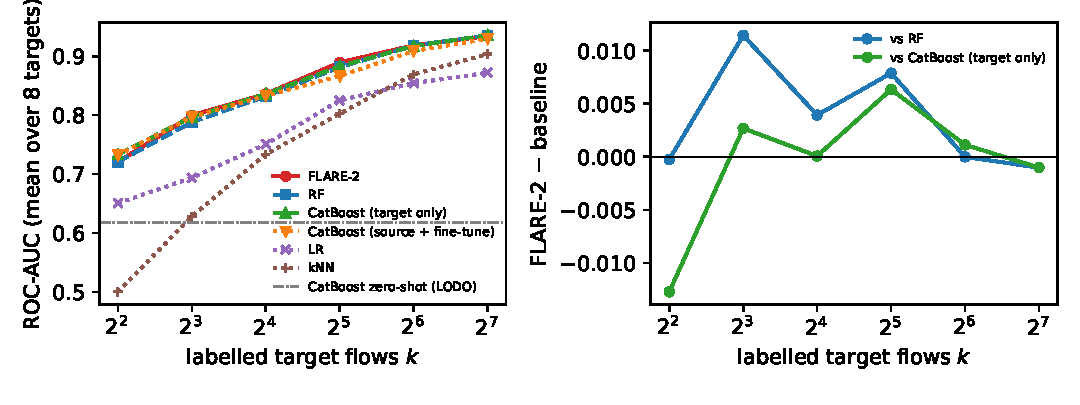
\includegraphics[width=\textwidth]{figures/curves.pdf}
\caption{Left: ROC-AUC against $k$, mean over the eight targets. Right: FLARE-2 minus RF and minus target-only CatBoost.}\label{fig:curves}
\end{figure}

\begin{table}[t]
\centering\small
\caption{Paired differences in binary ROC-AUC (FLARE-2 minus baseline), unit = target (8). W/L: targets where FLARE-2 is higher / lower. $p_{\text{Holm}}$: exact Wilcoxon over targets, Holm-adjusted over baselines.}\label{tab:stats}
\begin{tabular}{llcccc}
\toprule
Scope & Baseline & $\Delta$ROC-AUC & 95\% CI & W/L & $p_{\text{Holm}}$ \\
\midrule
mean over k & RF & +0.004 & [-0.003, +0.010] & 5/3 & 1.000 \\
mean over k & CatBoost (target) & -0.001 & [-0.004, +0.003] & 4/4 & 1.000 \\
mean over k & CatBoost (fine-tune) & +0.005 & [-0.010, +0.022] & 4/4 & 1.000 \\
mean over k & LR & +0.075 & [+0.044, +0.106] & 8/0 & 0.039 \\
mean over k & kNN & +0.110 & [+0.085, +0.133] & 8/0 & 0.039 \\
k$\leq$16 & RF & +0.005 & [-0.004, +0.014] & 4/4 & 1.000 \\
k$\leq$16 & CatBoost (target) & -0.003 & [-0.009, +0.002] & 4/4 & 1.000 \\
k$\leq$16 & CatBoost (fine-tune) & -0.002 & [-0.033, +0.030] & 4/4 & 1.000 \\
k$\leq$16 & LR & +0.087 & [+0.047, +0.128] & 8/0 & 0.039 \\
k$\leq$16 & kNN & +0.165 & [+0.121, +0.207] & 8/0 & 0.039 \\
k$\geq$32 & RF & +0.002 & [-0.003, +0.008] & 4/4 & 1.000 \\
k$\geq$32 & CatBoost (target) & +0.002 & [-0.002, +0.007] & 4/4 & 1.000 \\
k$\geq$32 & CatBoost (fine-tune) & +0.012 & [+0.006, +0.019] & 7/1 & 0.047 \\
k$\geq$32 & LR & +0.064 & [+0.034, +0.096] & 8/0 & 0.039 \\
k$\geq$32 & kNN & +0.056 & [+0.040, +0.073] & 8/0 & 0.039 \\
\bottomrule
\end{tabular}

\end{table}

Where FLARE-2 helps and where it does not is target-dependent (Fig.~\ref{fig:heat}).
It is ahead of RF at $k=4$ on CIC-IDS2017 ($+0.067$) and ahead at $k=8$--$16$ on InSDN and ToN-IoT, but behind at $k=4$ on InSDN, IoT-23 and UNSW-NB15 and behind at $k=16$ on USB-IDS-1 ($-0.036$) and CIC-IDS2017 ($-0.027$).
Targets whose attacks are easy (USB-IDS-1, where pooled zero-shot CatBoost already reaches 0.952) leave little to gain.

\begin{figure}[t]
\centering
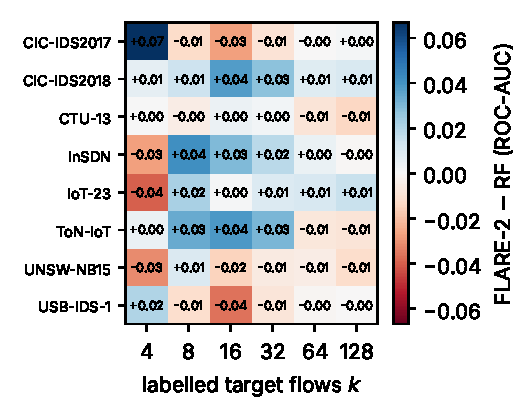
\includegraphics[width=0.55\textwidth]{figures/heatmap.pdf}
\caption{ROC-AUC difference FLARE-2 minus RF per target and $k$.}\label{fig:heat}
\end{figure}

\subsection{Comparison with a tabular foundation model}
Table~\ref{tab:binary} includes TabPFN-3.5.
On seed 0 the mean ROC-AUC over targets and $k$ is 0.862 for TabPFN-3.5, 0.857 for TabPFN-3, 0.850 for FLARE-2 and for target-only CatBoost, 0.846 for RF.
TabPFN-3.5 is higher than FLARE-2 on all 8 targets ($-0.012$ for FLARE-2 minus TabPFN-3.5, $p_{\text{Holm}}=0.016$ over the two versions; TabPFN-3: $-0.008$, $p_{\text{Holm}}=0.016$), and the 3-seed difference to TabPFN-3.5 is $-0.014$ (95\% interval $[-0.018,-0.011]$, 0 of 8 targets in favour of FLARE-2, standard deviation over seeds 0.002; Table~\ref{tab:tabpfn}).
The sign holds for the mean over targets at every $k$ and in both ranges ($k\le16$: $-0.016$; $k\ge32$: $-0.013$ over three seeds), although FLARE-2 is higher on 2 of 8 targets at some single values of $k$.
TabPFN-3.5 is also above the tree ensembles on seed 0 ($+0.016$ over RF on 8 of 8 targets, $+0.012$ over target-only CatBoost on 7 of 8, uncorrected $p=0.008$ and $0.016$; these comparisons were added after the five-baseline family of Table~\ref{tab:stats} was fixed) and not different from source-pretrained CatBoost ($+0.017$, 5 of 8 targets, $p=0.20$).
The differences are small in absolute terms (0.008 to 0.014 on average, 0.006 to 0.024 on individual targets for TabPFN-3.5 over three seeds), but consistent in sign for every target after averaging over $k$, and for every seed.
At $k=4$ all methods but LR and $k$NN are within 0.02 of each other (0.720 for FLARE-2, 0.736 for TabPFN-3.5).
TabPFN reads only the support rows while FLARE-2 additionally ranks features over the unlabelled target rows, so we do not expect the comparison to favour TabPFN: ranking over the support alone costs FLARE-2 only 0.007 ROC-AUC (Sect.~\ref{sec:controls}).
We do not know why meta-training on five or six real networks is not better than pretraining on a broad synthetic prior, and we have not tested explanations such as model scale, prior breadth or the number of meta-training datasets.

\begin{table}[t]
\centering\small
\caption{FLARE-2 minus TabPFN in binary ROC-AUC, unit = target (8). W/L: targets where FLARE-2 is higher / lower. Seed 0: $p_{\text{Holm}}$ over the two TabPFN versions within each scope. Three seeds: TabPFN-3.5 only, target-averaged over seeds 0--2, exact Wilcoxon $p$ without correction (rows marked 3 seeds). The last column is $p_{\text{Holm}}$ for seed 0 and uncorrected $p$ for three seeds.}\label{tab:tabpfn}
\begin{tabular}{llrrrr}
\toprule
Seeds & Baseline & Mean diff. & 95\% CI & W/L & p$_{\text{Holm}}$ \\
\midrule
mean over k & seed 0, TabPFN-3 & -0.008 & [-0.011, -0.005] & 0/8 & 0.016 \\
 & seed 0, TabPFN-3.5 & -0.012 & [-0.015, -0.009] & 0/8 & 0.016 \\
 & 3 seeds, TabPFN-3.5 & -0.014 & [-0.018, -0.011] & 0/8 & 0.008 \\
\midrule
k$\leq$16 & seed 0, TabPFN-3 & -0.008 & [-0.014, -0.002] & 1/7 & 0.055 \\
 & seed 0, TabPFN-3.5 & -0.014 & [-0.019, -0.009] & 1/7 & 0.031 \\
 & 3 seeds, TabPFN-3.5 & -0.016 & [-0.021, -0.012] & 0/8 & 0.008 \\
\midrule
k$\geq$32 & seed 0, TabPFN-3 & -0.008 & [-0.010, -0.005] & 0/8 & 0.016 \\
 & seed 0, TabPFN-3.5 & -0.010 & [-0.014, -0.007] & 0/8 & 0.016 \\
 & 3 seeds, TabPFN-3.5 & -0.013 & [-0.017, -0.009] & 0/8 & 0.008 \\
\bottomrule
\end{tabular}

\end{table}

\subsection{Attack-class level}
Table~\ref{tab:class} summarises per-class detection (class $c$ against benign, $k$ labelled flows of each) and $N$-way attack-type classification over 57 (target, class) detection tasks.
FLARE-2 has higher per-class ROC-AUC than RF and CatBoost on 7 of 8 targets (mean $+0.014$ and $+0.015$ over targets, $p=0.016$ before correction; the unit-level $p<0.001$ is optimistic because classes within a target are correlated).
It has a lower false-positive rate (by $0.05$; lower on 7 of 8 targets, $p=0.078$ at target level) and a lower recall (by $0.03$ to $0.04$; $p\le0.016$) at the default threshold of 0.5, so part of the ROC-AUC gain is a different operating point and not a free gain in detection.
Repeating the class-level evaluation with meta-training seeds 1 and 2 and averaging each target over the three seeds (Holm-adjusted over the four baselines, unit = target) gives the same picture with firmer tests: per-class ROC-AUC is higher than RF and CatBoost by $+0.011$ on 7 of 8 targets ($p_{\text{Holm}}=0.047$ for both), the false-positive rate is lower on 7 of 8 targets ($p_{\text{Holm}}=0.047$) and recall is lower on all 8 targets ($p_{\text{Holm}}=0.031$), so the operating-point caveat stands.
On $N$-way macro-F1, seed 0 gives $+0.026$ and $+0.022$ over RF and CatBoost (higher on 3 of 8 targets, $p=0.74$) and three seeds $+0.021$ and $+0.018$, which is not significant; FLARE-2 is significantly higher than LR and $k$NN.
$N$-way balanced accuracy, in contrast, is lower than CatBoost by $0.022$ (lower on 7 of 8 targets, $p_{\text{Holm}}=0.047$) and than RF by $0.023$ ($p_{\text{Holm}}=0.078$) over three seeds.
Per-target values are in Table~\ref{tab:classtarget}.

At class level TabPFN-3.5 is not better than FLARE-2 in ranking (Table~\ref{tab:tabpfnclass}): per-class ROC-AUC differs by $-0.002$ (95\% interval $[-0.014,+0.006]$, FLARE-2 higher on 4 of 8 targets) and $N$-way macro-F1 by $-0.014$ ($[-0.049,+0.019]$), neither significant, and the false-positive rate is not different.
TabPFN-3.5 has higher recall at the default threshold (by $0.043$ per class, 0 of 8 targets in favour of FLARE-2, $p_{\text{Holm}}=0.047$) and higher $N$-way balanced accuracy (by $0.048$, $p_{\text{Holm}}=0.078$), which is the same operating-point difference that FLARE-2 shows against the trees.
This comparison is seed 0 only, uses five draws, and, for five targets, a subsample of the query rows.

\begin{table}[t]
\centering\small
\caption{Class-level FLARE-2 minus TabPFN-3.5 (seed 0, $k\le16$ per class, five draws), unit = target (8). W/L: targets where FLARE-2 is higher / lower. $p$: exact Wilcoxon over targets, Holm-adjusted over the five metrics. For FPR a negative difference favours FLARE-2.}\label{tab:tabpfnclass}
\begin{tabular}{lrrrr}
\toprule
Metric & Mean diff. & 95\% CI & W/L & $p$ (Holm) \\
\midrule
Per-class ROC-AUC & -0.002 & [-0.014, +0.006] & 4/4 & 1.000 \\
Per-class FPR & -0.020 & [-0.050, +0.015] & 2/6 & 0.938 \\
Per-class recall & -0.043 & [-0.061, -0.025] & 0/8 & 0.047 \\
$N$-way macro-F1 & -0.014 & [-0.049, +0.019] & 3/5 & 1.000 \\
$N$-way balanced accuracy & -0.048 & [-0.070, -0.026] & 1/7 & 0.078 \\
\bottomrule
\end{tabular}

\end{table}

\begin{table}[t]
\centering\scriptsize
\caption{Class-level differences, FLARE-2 minus baseline. ``targets'': mean over the 8 targets of the target mean, count of targets where FLARE-2 is higher, exact Wilcoxon $p$ over targets (uncorrected). ``units'': mean over (target, class) pairs, $k\in\{2,4,8,16\}$ labelled flows per class. For FPR a negative difference favours FLARE-2.}\label{tab:class}
\begin{tabular}{llccccc}
\toprule
Metric & Baseline & $\Delta$ (targets) & FLARE-2 higher & $p$ & $\Delta$ (units) & units \\
\midrule
Per-class ROC-AUC & RF & +0.014 & 7/8 & 0.016 & +0.012 & 57 \\
Per-class ROC-AUC & CatBoost & +0.015 & 7/8 & 0.016 & +0.013 & 57 \\
Per-class ROC-AUC & LR & +0.082 & 8/8 & 0.008 & +0.075 & 57 \\
Per-class ROC-AUC & kNN & +0.175 & 8/8 & 0.008 & +0.167 & 57 \\
Per-class recall@0.5 & RF & -0.041 & 0/8 & 0.008 & -0.044 & 57 \\
Per-class recall@0.5 & CatBoost & -0.026 & 1/8 & 0.016 & -0.030 & 57 \\
Per-class recall@0.5 & LR & -0.025 & 2/8 & 0.078 & -0.030 & 57 \\
Per-class recall@0.5 & kNN & -0.048 & 1/8 & 0.023 & -0.056 & 57 \\
Per-class FPR@0.5 & RF & -0.053 & 1/8 & 0.078 & -0.052 & 57 \\
Per-class FPR@0.5 & CatBoost & -0.052 & 1/8 & 0.078 & -0.050 & 57 \\
Per-class FPR@0.5 & LR & -0.077 & 1/8 & 0.016 & -0.074 & 57 \\
Per-class FPR@0.5 & kNN & -0.334 & 0/8 & 0.008 & -0.330 & 57 \\
N-way macro-F1 & RF & +0.026 & 3/8 & 0.742 & +0.026 & 8 \\
N-way macro-F1 & CatBoost & +0.022 & 3/8 & 0.742 & +0.022 & 8 \\
N-way macro-F1 & LR & +0.074 & 7/8 & 0.016 & +0.074 & 8 \\
N-way macro-F1 & kNN & +0.127 & 8/8 & 0.008 & +0.127 & 8 \\
\bottomrule
\end{tabular}

\end{table}

\begin{table}[t]
\centering\small
\caption{Per-target class-level results. Left: per-class ROC-AUC at $k=4$ per class. Right: $N$-way macro-F1 at $k=16$ per class. InSDN is omitted because it has no class-level evaluation at $k=16$.}\label{tab:classtarget}
\begin{tabular}{lcccccc}
\toprule
& \multicolumn{3}{c}{Per-class ROC-AUC, $k{=}4$} & \multicolumn{3}{c}{N-way macro-F1, $k{=}16$} \\
\cmidrule(lr){2-4}\cmidrule(lr){5-7}
Target & F2 & RF & CB & F2 & RF & CB \\
\midrule
CIC-IDS2017 & \textbf{0.957} & 0.942 & 0.949 & \textbf{0.504} & 0.456 & 0.448 \\
CIC-IDS2018 & \textbf{0.889} & 0.879 & 0.875 & \textbf{0.658} & 0.517 & 0.582 \\
CTU-13 & \textbf{0.863} & 0.853 & 0.852 & \textbf{0.299} & 0.329 & 0.350 \\
IoT-23 & \textbf{0.879} & 0.842 & 0.841 & \textbf{0.644} & 0.562 & 0.589 \\
ToN-IoT & \textbf{0.927} & 0.906 & 0.925 & \textbf{0.680} & 0.705 & 0.688 \\
UNSW-NB15 & \textbf{0.857} & 0.845 & 0.839 & \textbf{0.294} & 0.337 & 0.323 \\
USB-IDS-1 & \textbf{0.995} & 0.998 & 0.999 & \textbf{0.461} & 0.461 & 0.468 \\
\bottomrule
\end{tabular}

\end{table}

\subsection{Ablations}
Ablations are running; this section is completed when they finish.


\section{Limitations}
\begin{itemize}
\item The main tables and figures use meta-training seed 0 with 10 support draws per target; seeds 1 and 2 were run for all targets and are summarised in Table~\ref{tab:seeds} and in the text for the class level (the class-level tables themselves are seed 0), and the ablations use one seed and two targets (the loss-mask comparison uses all eight targets, the controls the seed-1 models).
\item FLARE-2 is not better than fixed-setting tree ensembles on binary ROC-AUC, and TabPFN is better than FLARE-2 on every target; its remaining gains are class-level and conditional on the operating point.
\item The class-level TabPFN comparison is seed 0 only, with five draws and, for five of the eight targets, a stratified subsample of at most 5\,000 query rows per task (checked on one target: differences of at most 0.005).
\item The TabPFN comparison uses default settings, three seeds for version 3.5 and one for version 3, and the released weights under a non-commercial license; a tuned or fine-tuned TabPFN, or a tuned FLARE-2, could change the gaps, which are 0.008 to 0.014 ROC-AUC on average.
\item Eight datasets from five laboratories (UNB, Sannio, UCD, UNSW, CTU), so datasets are not independent units; results on other networks may differ.
\item FLARE-2 normalises features by rank over the unlabelled target rows it scores, which is transductive in the target features (a 256-row query reference gives the same ROC-AUC and support-only ranks lower it by 0.007, Sect.~\ref{sec:controls}), and the baselines get no such information; one meta-trained model per target is needed (leave-one-dataset-out), and each model sees only five or six training datasets. All eight targets were used while choosing the architecture and the task mix, so there is no untouched test set. Source-pretrained CatBoost is better than FLARE-2 at $k=4$ on four targets.
\item Queries whose class has no support row (label noise at $k=1$) receive a target logit of $-10^{9}$. This produced training losses of order $10^{6}$ and, in one binary-only ablation run, made validation loss pick a collapsed checkpoint (AUC about 0.50); checkpoint selection now scores supported queries only. The checkpoint selection of the main FLARE-2 runs is unaffected (their validation episodes contained no unsupported queries), but their training loss includes these queries (logged loss of order $10^{6}$ to $10^{7}$). The loss-masked variant, trained on all eight targets with seed 0, has mean binary ROC-AUC 0.851 against 0.850 for FLARE-2, with per-target differences between $-0.010$ and $+0.019$ and a gain on 4 of 8 targets (Sect.~\ref{sec:ablation}).
\item Flows only; payload features and temporal context are not used.
\item The datasets are public laboratory captures with their own labelling errors \citep{engelen2021troubleshooting}.
\end{itemize}

\section{Conclusion}
Concept shift, rather than tuning, appears to limit cross-dataset flow classification, so a model that carries a fixed decision function across networks is a poor target.
What source data can still provide is a prior over how to learn a rule from a few labelled flows.
FLARE-2, a transformer meta-trained on real network tasks, matches fixed-setting tree ensembles on binary detection without fitting the network to the target and modestly improves per-class ranking over the trees (but not over TabPFN-3.5, which also has higher recall), while a general tabular foundation model, TabPFN versions 3 and 3.5, is better on every target (mean over $k$) by 0.008 (version 3, seed 0) to 0.014 (version 3.5, three seeds) ROC-AUC without any training or tuning on network data by us.
The practical conclusion is that labelled flows from the target network, read by a strong pretrained prior, are what works, and that in our experiments meta-training on a handful of real networks did not improve on that prior.
Open problems are the gap to full-label training (0.95--1.00 ROC-AUC) at small $k$, tuning and fine-tuning the foundation model, and testing whether a meta-trainer with more networks, more steps or a larger model closes the gap.

\paragraph{Reproducibility.}
The package, configurations, sampled-row hashes and every raw per-run CSV are in \url{https://github.com/vinhqdang/cross_ids}; tables and figures are generated by \texttt{scripts/make\_paper\_tables.py} and statistics by \texttt{scripts/stats\_flare.py}.

\bibliographystyle{plainnat}
\bibliography{refs}
\end{document}
